\documentclass[1p]{elsarticle_modified}
%\bibliographystyle{elsarticle-num}

%\usepackage[colorlinks]{hyperref}
%\usepackage{abbrmath_seonhwa} %\Abb, \Ascr, \Acal ,\Abf, \Afrak
\usepackage{amsfonts}
\usepackage{amssymb}
\usepackage{amsmath}
\usepackage{amsthm}
\usepackage{scalefnt}
\usepackage{amsbsy}
\usepackage{kotex}
\usepackage{caption}
\usepackage{subfig}
\usepackage{color}
\usepackage{graphicx}
\usepackage{xcolor} %% white, black, red, green, blue, cyan, magenta, yellow
\usepackage{float}
\usepackage{setspace}
\usepackage{hyperref}

\usepackage{tikz}
\usetikzlibrary{arrows}

\usepackage{multirow}
\usepackage{array} % fixed length table
\usepackage{hhline}

%%%%%%%%%%%%%%%%%%%%%
\makeatletter
\renewcommand*\env@matrix[1][\arraystretch]{%
	\edef\arraystretch{#1}%
	\hskip -\arraycolsep
	\let\@ifnextchar\new@ifnextchar
	\array{*\c@MaxMatrixCols c}}
\makeatother %https://tex.stackexchange.com/questions/14071/how-can-i-increase-the-line-spacing-in-a-matrix
%%%%%%%%%%%%%%%

\usepackage[normalem]{ulem}

\newcommand{\msout}[1]{\ifmmode\text{\sout{\ensuremath{#1}}}\else\sout{#1}\fi}
%SOURCE: \msout is \stkout macro in https://tex.stackexchange.com/questions/20609/strikeout-in-math-mode

\newcommand{\cancel}[1]{
	\ifmmode
	{\color{red}\msout{#1}}
	\else
	{\color{red}\sout{#1}}
	\fi
}

\newcommand{\add}[1]{
	{\color{blue}\uwave{#1}}
}

\newcommand{\replace}[2]{
	\ifmmode
	{\color{red}\msout{#1}}{\color{blue}\uwave{#2}}
	\else
	{\color{red}\sout{#1}}{\color{blue}\uwave{#2}}
	\fi
}

\newcommand{\Sol}{\mathcal{S}} %segment
\newcommand{\D}{D} %diagram
\newcommand{\A}{\mathcal{A}} %arc


%%%%%%%%%%%%%%%%%%%%%%%%%%%%%5 test

\def\sl{\operatorname{\textup{SL}}(2,\Cbb)}
\def\psl{\operatorname{\textup{PSL}}(2,\Cbb)}
\def\quan{\mkern 1mu \triangleright \mkern 1mu}

\theoremstyle{definition}
\newtheorem{thm}{Theorem}[section]
\newtheorem{prop}[thm]{Proposition}
\newtheorem{lem}[thm]{Lemma}
\newtheorem{ques}[thm]{Question}
\newtheorem{cor}[thm]{Corollary}
\newtheorem{defn}[thm]{Definition}
\newtheorem{exam}[thm]{Example}
\newtheorem{rmk}[thm]{Remark}
\newtheorem{alg}[thm]{Algorithm}

\newcommand{\I}{\sqrt{-1}}
\begin{document}

%\begin{frontmatter}
%
%\title{Boundary parabolic representations of knots up to 8 crossings}
%
%%% Group authors per affiliation:
%\author{Yunhi Cho} 
%\address{Department of Mathematics, University of Seoul, Seoul, Korea}
%\ead{yhcho@uos.ac.kr}
%
%
%\author{Seonhwa Kim} %\fnref{s_kim}}
%\address{Center for Geometry and Physics, Institute for Basic Science, Pohang, 37673, Korea}
%\ead{ryeona17@ibs.re.kr}
%
%\author{Hyuk Kim}
%\address{Department of Mathematical Sciences, Seoul National University, Seoul 08826, Korea}
%\ead{hyukkim@snu.ac.kr}
%
%\author{Seokbeom Yoon}
%\address{Department of Mathematical Sciences, Seoul National University, Seoul, 08826,  Korea}
%\ead{sbyoon15@snu.ac.kr}
%
%\begin{abstract}
%We find all boundary parabolic representation of knots up to 8 crossings.
%
%\end{abstract}
%\begin{keyword}
%    \MSC[2010] 57M25 
%\end{keyword}
%
%\end{frontmatter}

%\linenumbers
%\tableofcontents
%
\newcommand\colored[1]{\textcolor{white}{\rule[-0.35ex]{0.8em}{1.4ex}}\kern-0.8em\color{red} #1}%
%\newcommand\colored[1]{\textcolor{white}{ #1}\kern-2.17ex	\textcolor{white}{ #1}\kern-1.81ex	\textcolor{white}{ #1}\kern-2.15ex\color{red}#1	}

{\Large $\underline{12n_{0679}~(K12n_{0679})}$}

\setlength{\tabcolsep}{10pt}
\renewcommand{\arraystretch}{1.6}
\vspace{1cm}\begin{tabular}{m{100pt}>{\centering\arraybackslash}m{274pt}}
\multirow{5}{120pt}{
	\centering
	\includegraphics[width=112pt]{../../../GIT/diagram.site/Diagrams/png/2768_12n_0679.png}\\
\ \ \ A knot diagram\footnotemark}&
\allowdisplaybreaks
\textbf{Linearized knot diagam} \\
\cline{2-2}
 &
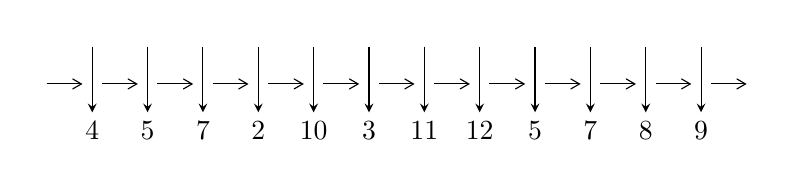
\begin{tikzpicture}[x=20pt, y=17pt]
	% nodes
	\node (C0) at (0, 0) {};
	\node (C1) at (1, 0) {};
	\node (C1U) at (1, +1) {};
	\node (C1D) at (1, -1) {4};

	\node (C2) at (2, 0) {};
	\node (C2U) at (2, +1) {};
	\node (C2D) at (2, -1) {5};

	\node (C3) at (3, 0) {};
	\node (C3U) at (3, +1) {};
	\node (C3D) at (3, -1) {7};

	\node (C4) at (4, 0) {};
	\node (C4U) at (4, +1) {};
	\node (C4D) at (4, -1) {2};

	\node (C5) at (5, 0) {};
	\node (C5U) at (5, +1) {};
	\node (C5D) at (5, -1) {10};

	\node (C6) at (6, 0) {};
	\node (C6U) at (6, +1) {};
	\node (C6D) at (6, -1) {3};

	\node (C7) at (7, 0) {};
	\node (C7U) at (7, +1) {};
	\node (C7D) at (7, -1) {11};

	\node (C8) at (8, 0) {};
	\node (C8U) at (8, +1) {};
	\node (C8D) at (8, -1) {12};

	\node (C9) at (9, 0) {};
	\node (C9U) at (9, +1) {};
	\node (C9D) at (9, -1) {5};

	\node (C10) at (10, 0) {};
	\node (C10U) at (10, +1) {};
	\node (C10D) at (10, -1) {7};

	\node (C11) at (11, 0) {};
	\node (C11U) at (11, +1) {};
	\node (C11D) at (11, -1) {8};

	\node (C12) at (12, 0) {};
	\node (C12U) at (12, +1) {};
	\node (C12D) at (12, -1) {9};
	\node (C13) at (13, 0) {};

	% arrows
	\draw[->,>={angle 60}]
	(C0) edge (C1) (C1) edge (C2) (C2) edge (C3) (C3) edge (C4) (C4) edge (C5) (C5) edge (C6) (C6) edge (C7) (C7) edge (C8) (C8) edge (C9) (C9) edge (C10) (C10) edge (C11) (C11) edge (C12) (C12) edge (C13) ;	\draw[->,>=stealth]
	(C1U) edge (C1D) (C2U) edge (C2D) (C3U) edge (C3D) (C4U) edge (C4D) (C5U) edge (C5D) (C6U) edge (C6D) (C7U) edge (C7D) (C8U) edge (C8D) (C9U) edge (C9D) (C10U) edge (C10D) (C11U) edge (C11D) (C12U) edge (C12D) ;
	\end{tikzpicture} \\
\hhline{~~} \\& 
\textbf{Solving Sequence} \\ \cline{2-2} 
 &
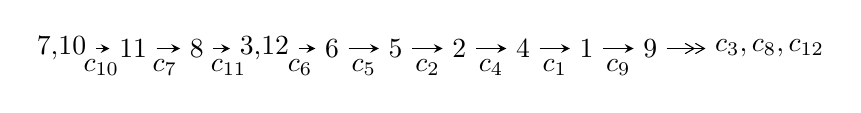
\begin{tikzpicture}[x=23pt, y=7pt]
	% node
	\node (A0) at (-1/8, 0) {7,10};
	\node (A1) at (1, 0) {11};
	\node (A2) at (2, 0) {8};
	\node (A3) at (49/16, 0) {3,12};
	\node (A4) at (33/8, 0) {6};
	\node (A5) at (41/8, 0) {5};
	\node (A6) at (49/8, 0) {2};
	\node (A7) at (57/8, 0) {4};
	\node (A8) at (65/8, 0) {1};
	\node (A9) at (73/8, 0) {9};
	\node (C1) at (1/2, -1) {$c_{10}$};
	\node (C2) at (3/2, -1) {$c_{7}$};
	\node (C3) at (5/2, -1) {$c_{11}$};
	\node (C4) at (29/8, -1) {$c_{6}$};
	\node (C5) at (37/8, -1) {$c_{5}$};
	\node (C6) at (45/8, -1) {$c_{2}$};
	\node (C7) at (53/8, -1) {$c_{4}$};
	\node (C8) at (61/8, -1) {$c_{1}$};
	\node (C9) at (69/8, -1) {$c_{9}$};
	\node (A10) at (11, 0) {$c_{3},c_{8},c_{12}$};

	% edge
	\draw[->,>=stealth]	
	(A0) edge (A1) (A1) edge (A2) (A2) edge (A3) (A3) edge (A4) (A4) edge (A5) (A5) edge (A6) (A6) edge (A7) (A7) edge (A8) (A8) edge (A9) ;
	\draw[->>,>={angle 60}]	
	(A9) edge (A10);
\end{tikzpicture} \\ 

\end{tabular} \\

\footnotetext{
The image of knot diagram is generated by the software ``\textbf{Draw programme}" developed by Andrew Bartholomew(\url{http://www.layer8.co.uk/maths/draw/index.htm\#Running-draw}), where we modified some parts for our purpose(\url{https://github.com/CATsTAILs/LinksPainter}).
}\phantom \\ \newline 
\centering \textbf{Ideals for irreducible components\footnotemark of $X_{\text{par}}$} 
 
\begin{align*}
I^u_{1}&=\langle 
-272506 u^{18}-964931 u^{17}+\cdots+166246 b-454705,\\
\phantom{I^u_{1}}&\phantom{= \langle  }202199 u^{18}+697603 u^{17}+\cdots+166246 a+690296,\;u^{19}+4 u^{18}+\cdots+6 u+1\rangle \\
I^u_{2}&=\langle 
u^2+b+u-2,\;a,\;u^3+u^2-2 u-1\rangle \\
I^u_{3}&=\langle 
b-1,\;a+1,\;u^2- u-1\rangle \\
I^u_{4}&=\langle 
b+u+1,\;a+u-2,\;u^2- u-1\rangle \\
\\
\end{align*}
\raggedright * 4 irreducible components of $\dim_{\mathbb{C}}=0$, with total 26 representations.\\
\footnotetext{All coefficients of polynomials are rational numbers. But the coefficients are sometimes approximated in decimal forms when there is not enough margin.}
\newpage
\renewcommand{\arraystretch}{1}
\centering \section*{I. $I^u_{1}= \langle -2.73\times10^{5} u^{18}-9.65\times10^{5} u^{17}+\cdots+1.66\times10^{5} b-4.55\times10^{5},\;2.02\times10^{5} u^{18}+6.98\times10^{5} u^{17}+\cdots+1.66\times10^{5} a+6.90\times10^{5},\;u^{19}+4 u^{18}+\cdots+6 u+1 \rangle$}
\flushleft \textbf{(i) Arc colorings}\\
\begin{tabular}{m{7pt} m{180pt} m{7pt} m{180pt} }
\flushright $a_{7}=$&$\begin{pmatrix}0\\u\end{pmatrix}$ \\
\flushright $a_{10}=$&$\begin{pmatrix}1\\0\end{pmatrix}$ \\
\flushright $a_{11}=$&$\begin{pmatrix}1\\u^2\end{pmatrix}$ \\
\flushright $a_{8}=$&$\begin{pmatrix}- u\\- u^3+u\end{pmatrix}$ \\
\flushright $a_{3}=$&$\begin{pmatrix}-1.21626 u^{18}-4.19621 u^{17}+\cdots-17.4998 u-4.15226\\1.63917 u^{18}+5.80424 u^{17}+\cdots+13.5564 u+2.73513\end{pmatrix}$ \\
\flushright $a_{12}=$&$\begin{pmatrix}- u^2+1\\- u^4+2 u^2\end{pmatrix}$ \\
\flushright $a_{6}=$&$\begin{pmatrix}-1.42025 u^{18}-4.28958 u^{17}+\cdots-12.9625 u-2.68015\\0.636515 u^{18}+1.48579 u^{17}+\cdots+2.46235 u-0.167595\end{pmatrix}$ \\
\flushright $a_{5}=$&$\begin{pmatrix}-0.783736 u^{18}-2.80379 u^{17}+\cdots-10.5002 u-2.84774\\0.636515 u^{18}+1.48579 u^{17}+\cdots+2.46235 u-0.167595\end{pmatrix}$ \\
\flushright $a_{2}=$&$\begin{pmatrix}-0.783736 u^{18}-2.80379 u^{17}+\cdots-10.5002 u-2.84774\\0.912202 u^{18}+3.77581 u^{17}+\cdots+10.4811 u+2.39994\end{pmatrix}$ \\
\flushright $a_{4}=$&$\begin{pmatrix}-1.21626 u^{18}-4.19621 u^{17}+\cdots-17.4998 u-4.15226\\0.949954 u^{18}+3.82918 u^{17}+\cdots+10.7596 u+2.06629\end{pmatrix}$ \\
\flushright $a_{1}=$&$\begin{pmatrix}- u^4+3 u^2-1\\- u^6+4 u^4-3 u^2\end{pmatrix}$ \\
\flushright $a_{9}=$&$\begin{pmatrix}u^3-2 u\\u^5-3 u^3+u\end{pmatrix}$\\&\end{tabular}
\flushleft \textbf{(ii) Obstruction class $= -1$}\\~\\
\flushleft \textbf{(iii) Cusp Shapes $= \frac{6730797}{166246} u^{18}+\frac{11675065}{83123} u^{17}+\cdots+\frac{25540453}{83123} u+\frac{10182639}{166246}$}\\~\\
\newpage\renewcommand{\arraystretch}{1}
\flushleft \textbf{(iv) u-Polynomials at the component}\newline \\
\begin{tabular}{m{50pt}|m{274pt}}
Crossings & \hspace{64pt}u-Polynomials at each crossing \\
\hline $$\begin{aligned}c_{1},c_{2},c_{4}\end{aligned}$$&$\begin{aligned}
&u^{19}-6 u^{18}+\cdots+15 u+1
\end{aligned}$\\
\hline $$\begin{aligned}c_{3},c_{6}\end{aligned}$$&$\begin{aligned}
&u^{19}+3 u^{18}+\cdots+4 u+8
\end{aligned}$\\
\hline $$\begin{aligned}c_{5},c_{9}\end{aligned}$$&$\begin{aligned}
&u^{19}-2 u^{18}+\cdots+32 u+16
\end{aligned}$\\
\hline $$\begin{aligned}c_{7},c_{8},c_{10}\\c_{11},c_{12}\end{aligned}$$&$\begin{aligned}
&u^{19}+4 u^{18}+\cdots+6 u+1
\end{aligned}$\\
\hline
\end{tabular}\\~\\
\newpage\renewcommand{\arraystretch}{1}
\flushleft \textbf{(v) Riley Polynomials at the component}\newline \\
\begin{tabular}{m{50pt}|m{274pt}}
Crossings & \hspace{64pt}Riley Polynomials at each crossing \\
\hline $$\begin{aligned}c_{1},c_{2},c_{4}\end{aligned}$$&$\begin{aligned}
&y^{19}-8 y^{18}+\cdots+227 y-1
\end{aligned}$\\
\hline $$\begin{aligned}c_{3},c_{6}\end{aligned}$$&$\begin{aligned}
&y^{19}+15 y^{18}+\cdots+2448 y-64
\end{aligned}$\\
\hline $$\begin{aligned}c_{5},c_{9}\end{aligned}$$&$\begin{aligned}
&y^{19}+20 y^{18}+\cdots+6272 y-256
\end{aligned}$\\
\hline $$\begin{aligned}c_{7},c_{8},c_{10}\\c_{11},c_{12}\end{aligned}$$&$\begin{aligned}
&y^{19}-22 y^{18}+\cdots-6 y-1
\end{aligned}$\\
\hline
\end{tabular}\\~\\
\newpage\flushleft \textbf{(vi) Complex Volumes and Cusp Shapes}
$$\begin{array}{c|c|c}  
\text{Solutions to }I^u_{1}& \I (\text{vol} + \sqrt{-1}CS) & \text{Cusp shape}\\
 \hline 
\begin{aligned}
u &= \phantom{-}0.371183 + 0.912603 I \\
a &= -1.80989 - 0.68295 I \\
b &= \phantom{-}1.53400 + 0.07023 I\end{aligned}
 & \phantom{-}6.24887 + 1.03604 I & -13.20409 - 0.16139 I \\ \hline\begin{aligned}
u &= \phantom{-}0.371183 - 0.912603 I \\
a &= -1.80989 + 0.68295 I \\
b &= \phantom{-}1.53400 - 0.07023 I\end{aligned}
 & \phantom{-}6.24887 - 1.03604 I & -13.20409 + 0.16139 I \\ \hline\begin{aligned}
u &= \phantom{-}0.754085 + 0.801793 I \\
a &= \phantom{-}1.59489 + 0.69061 I \\
b &= -1.59706 + 0.29496 I\end{aligned}
 & \phantom{-}5.09846 - 6.69074 I & -15.1331 + 4.7970 I \\ \hline\begin{aligned}
u &= \phantom{-}0.754085 - 0.801793 I \\
a &= \phantom{-}1.59489 - 0.69061 I \\
b &= -1.59706 - 0.29496 I\end{aligned}
 & \phantom{-}5.09846 + 6.69074 I & -15.1331 - 4.7970 I \\ \hline\begin{aligned}
u &= \phantom{-}0.788633\phantom{ +0.000000I} \\
a &= -1.87771\phantom{ +0.000000I} \\
b &= \phantom{-}0.117506\phantom{ +0.000000I}\end{aligned}
 & -10.1632\phantom{ +0.000000I} & -31.8240\phantom{ +0.000000I} \\ \hline\begin{aligned}
u &= -1.296690 + 0.113032 I \\
a &= -0.844571 - 0.789505 I \\
b &= \phantom{-}1.171320 + 0.089530 I\end{aligned}
 & -4.61857 + 1.71767 I & -18.2481 - 1.2911 I \\ \hline\begin{aligned}
u &= -1.296690 - 0.113032 I \\
a &= -0.844571 + 0.789505 I \\
b &= \phantom{-}1.171320 - 0.089530 I\end{aligned}
 & -4.61857 - 1.71767 I & -18.2481 + 1.2911 I \\ \hline\begin{aligned}
u &= -0.541707\phantom{ +0.000000I} \\
a &= \phantom{-}0.445654\phantom{ +0.000000I} \\
b &= -3.62686\phantom{ +0.000000I}\end{aligned}
 & -2.44677\phantom{ +0.000000I} & -98.2800\phantom{ +0.000000I} \\ \hline\begin{aligned}
u &= -1.44566 + 0.37064 I \\
a &= \phantom{-}0.833635 - 0.884796 I \\
b &= -1.51545 - 0.17161 I\end{aligned}
 & \phantom{-}0.51136 + 3.59146 I & -15.7311 - 1.9367 I \\ \hline\begin{aligned}
u &= -1.44566 - 0.37064 I \\
a &= \phantom{-}0.833635 + 0.884796 I \\
b &= -1.51545 + 0.17161 I\end{aligned}
 & \phantom{-}0.51136 - 3.59146 I & -15.7311 + 1.9367 I\\
 \hline 
 \end{array}$$\newpage$$\begin{array}{c|c|c}  
\text{Solutions to }I^u_{1}& \I (\text{vol} + \sqrt{-1}CS) & \text{Cusp shape}\\
 \hline 
\begin{aligned}
u &= \phantom{-}1.49235 + 0.21013 I \\
a &= \phantom{-}0.018135 - 0.695055 I \\
b &= \phantom{-}0.526738 - 0.141756 I\end{aligned}
 & -6.67966 - 1.72802 I & -16.2689 + 1.8813 I \\ \hline\begin{aligned}
u &= \phantom{-}1.49235 - 0.21013 I \\
a &= \phantom{-}0.018135 + 0.695055 I \\
b &= \phantom{-}0.526738 + 0.141756 I\end{aligned}
 & -6.67966 + 1.72802 I & -16.2689 - 1.8813 I \\ \hline\begin{aligned}
u &= \phantom{-}1.60645\phantom{ +0.000000I} \\
a &= -0.333194\phantom{ +0.000000I} \\
b &= \phantom{-}3.67997\phantom{ +0.000000I}\end{aligned}
 & -10.0473\phantom{ +0.000000I} & -54.2350\phantom{ +0.000000I} \\ \hline\begin{aligned}
u &= -0.369925\phantom{ +0.000000I} \\
a &= -0.699220\phantom{ +0.000000I} \\
b &= -0.403627\phantom{ +0.000000I}\end{aligned}
 & -0.654259\phantom{ +0.000000I} & -14.8880\phantom{ +0.000000I} \\ \hline\begin{aligned}
u &= -1.65257 + 0.26840 I \\
a &= -0.793286 + 0.765963 I \\
b &= \phantom{-}1.67968 + 0.52712 I\end{aligned}
 & -2.92778 + 10.79900 I & -18.2574 - 5.0475 I \\ \hline\begin{aligned}
u &= -1.65257 - 0.26840 I \\
a &= -0.793286 - 0.765963 I \\
b &= \phantom{-}1.67968 - 0.52712 I\end{aligned}
 & -2.92778 - 10.79900 I & -18.2574 + 5.0475 I \\ \hline\begin{aligned}
u &= -0.082620 + 0.268767 I \\
a &= -0.49970 - 2.54134 I \\
b &= -0.546098 + 0.125693 I\end{aligned}
 & -0.761541 - 0.128012 I & -12.14415 - 0.42322 I \\ \hline\begin{aligned}
u &= -0.082620 - 0.268767 I \\
a &= -0.49970 + 2.54134 I \\
b &= -0.546098 - 0.125693 I\end{aligned}
 & -0.761541 + 0.128012 I & -12.14415 + 0.42322 I \\ \hline\begin{aligned}
u &= -1.76360\phantom{ +0.000000I} \\
a &= \phantom{-}0.466063\phantom{ +0.000000I} \\
b &= -0.273248\phantom{ +0.000000I}\end{aligned}
 & \phantom{-}19.6998\phantom{ +0.000000I} & -27.7990\phantom{ +0.000000I}\\
 \hline 
 \end{array}$$\newpage\newpage\renewcommand{\arraystretch}{1}
\centering \section*{II. $I^u_{2}= \langle u^2+b+u-2,\;a,\;u^3+u^2-2 u-1 \rangle$}
\flushleft \textbf{(i) Arc colorings}\\
\begin{tabular}{m{7pt} m{180pt} m{7pt} m{180pt} }
\flushright $a_{7}=$&$\begin{pmatrix}0\\u\end{pmatrix}$ \\
\flushright $a_{10}=$&$\begin{pmatrix}1\\0\end{pmatrix}$ \\
\flushright $a_{11}=$&$\begin{pmatrix}1\\u^2\end{pmatrix}$ \\
\flushright $a_{8}=$&$\begin{pmatrix}- u\\u^2- u-1\end{pmatrix}$ \\
\flushright $a_{3}=$&$\begin{pmatrix}0\\- u^2- u+2\end{pmatrix}$ \\
\flushright $a_{12}=$&$\begin{pmatrix}- u^2+1\\- u^2+u+1\end{pmatrix}$ \\
\flushright $a_{6}=$&$\begin{pmatrix}0\\u\end{pmatrix}$ \\
\flushright $a_{5}=$&$\begin{pmatrix}u\\u\end{pmatrix}$ \\
\flushright $a_{2}=$&$\begin{pmatrix}- u\\- u^2-2 u+2\end{pmatrix}$ \\
\flushright $a_{4}=$&$\begin{pmatrix}0\\- u^2- u+2\end{pmatrix}$ \\
\flushright $a_{1}=$&$\begin{pmatrix}- u\\- u\end{pmatrix}$ \\
\flushright $a_{9}=$&$\begin{pmatrix}- u^2+1\\- u^2\end{pmatrix}$\\&\end{tabular}
\flushleft \textbf{(ii) Obstruction class $= 1$}\\~\\
\flushleft \textbf{(iii) Cusp Shapes $= -8 u^2-7 u+2$}\\~\\
\newpage\renewcommand{\arraystretch}{1}
\flushleft \textbf{(iv) u-Polynomials at the component}\newline \\
\begin{tabular}{m{50pt}|m{274pt}}
Crossings & \hspace{64pt}u-Polynomials at each crossing \\
\hline $$\begin{aligned}c_{1},c_{2}\end{aligned}$$&$\begin{aligned}
&(u-1)^3
\end{aligned}$\\
\hline $$\begin{aligned}c_{3},c_{6}\end{aligned}$$&$\begin{aligned}
&u^3
\end{aligned}$\\
\hline $$\begin{aligned}c_{4}\end{aligned}$$&$\begin{aligned}
&(u+1)^3
\end{aligned}$\\
\hline $$\begin{aligned}c_{5},c_{7},c_{8}\end{aligned}$$&$\begin{aligned}
&u^3- u^2-2 u+1
\end{aligned}$\\
\hline $$\begin{aligned}c_{9},c_{10},c_{11}\\c_{12}\end{aligned}$$&$\begin{aligned}
&u^3+u^2-2 u-1
\end{aligned}$\\
\hline
\end{tabular}\\~\\
\newpage\renewcommand{\arraystretch}{1}
\flushleft \textbf{(v) Riley Polynomials at the component}\newline \\
\begin{tabular}{m{50pt}|m{274pt}}
Crossings & \hspace{64pt}Riley Polynomials at each crossing \\
\hline $$\begin{aligned}c_{1},c_{2},c_{4}\end{aligned}$$&$\begin{aligned}
&(y-1)^3
\end{aligned}$\\
\hline $$\begin{aligned}c_{3},c_{6}\end{aligned}$$&$\begin{aligned}
&y^3
\end{aligned}$\\
\hline $$\begin{aligned}c_{5},c_{7},c_{8}\\c_{9},c_{10},c_{11}\\c_{12}\end{aligned}$$&$\begin{aligned}
&y^3-5 y^2+6 y-1
\end{aligned}$\\
\hline
\end{tabular}\\~\\
\newpage\flushleft \textbf{(vi) Complex Volumes and Cusp Shapes}
$$\begin{array}{c|c|c}  
\text{Solutions to }I^u_{2}& \I (\text{vol} + \sqrt{-1}CS) & \text{Cusp shape}\\
 \hline 
\begin{aligned}
u &= \phantom{-}1.24698\phantom{ +0.000000I} \\
a &= \phantom{-0.000000 } 0 \\
b &= -0.801938\phantom{ +0.000000I}\end{aligned}
 & -7.98968\phantom{ +0.000000I} & -19.1690\phantom{ +0.000000I} \\ \hline\begin{aligned}
u &= -0.445042\phantom{ +0.000000I} \\
a &= \phantom{-0.000000 } 0 \\
b &= \phantom{-}2.24698\phantom{ +0.000000I}\end{aligned}
 & -2.34991\phantom{ +0.000000I} & \phantom{-}3.53080\phantom{ +0.000000I} \\ \hline\begin{aligned}
u &= -1.80194\phantom{ +0.000000I} \\
a &= \phantom{-0.000000 } 0 \\
b &= \phantom{-}0.554958\phantom{ +0.000000I}\end{aligned}
 & -19.2692\phantom{ +0.000000I} & -11.3620\phantom{ +0.000000I}\\
 \hline 
 \end{array}$$\newpage\newpage\renewcommand{\arraystretch}{1}
\centering \section*{III. $I^u_{3}= \langle b-1,\;a+1,\;u^2- u-1 \rangle$}
\flushleft \textbf{(i) Arc colorings}\\
\begin{tabular}{m{7pt} m{180pt} m{7pt} m{180pt} }
\flushright $a_{7}=$&$\begin{pmatrix}0\\u\end{pmatrix}$ \\
\flushright $a_{10}=$&$\begin{pmatrix}1\\0\end{pmatrix}$ \\
\flushright $a_{11}=$&$\begin{pmatrix}1\\u+1\end{pmatrix}$ \\
\flushright $a_{8}=$&$\begin{pmatrix}- u\\- u-1\end{pmatrix}$ \\
\flushright $a_{3}=$&$\begin{pmatrix}-1\\1\end{pmatrix}$ \\
\flushright $a_{12}=$&$\begin{pmatrix}- u\\- u\end{pmatrix}$ \\
\flushright $a_{6}=$&$\begin{pmatrix}u\\0\end{pmatrix}$ \\
\flushright $a_{5}=$&$\begin{pmatrix}u\\0\end{pmatrix}$ \\
\flushright $a_{2}=$&$\begin{pmatrix}u\\1\end{pmatrix}$ \\
\flushright $a_{4}=$&$\begin{pmatrix}-1\\- u\end{pmatrix}$ \\
\flushright $a_{1}=$&$\begin{pmatrix}0\\- u\end{pmatrix}$ \\
\flushright $a_{9}=$&$\begin{pmatrix}1\\0\end{pmatrix}$\\&\end{tabular}
\flushleft \textbf{(ii) Obstruction class $= 1$}\\~\\
\flushleft \textbf{(iii) Cusp Shapes $= -19$}\\~\\
\newpage\renewcommand{\arraystretch}{1}
\flushleft \textbf{(iv) u-Polynomials at the component}\newline \\
\begin{tabular}{m{50pt}|m{274pt}}
Crossings & \hspace{64pt}u-Polynomials at each crossing \\
\hline $$\begin{aligned}c_{1},c_{2},c_{3}\\c_{7},c_{8}\end{aligned}$$&$\begin{aligned}
&u^2+u-1
\end{aligned}$\\
\hline $$\begin{aligned}c_{4},c_{6},c_{10}\\c_{11},c_{12}\end{aligned}$$&$\begin{aligned}
&u^2- u-1
\end{aligned}$\\
\hline $$\begin{aligned}c_{5},c_{9}\end{aligned}$$&$\begin{aligned}
&u^2
\end{aligned}$\\
\hline
\end{tabular}\\~\\
\newpage\renewcommand{\arraystretch}{1}
\flushleft \textbf{(v) Riley Polynomials at the component}\newline \\
\begin{tabular}{m{50pt}|m{274pt}}
Crossings & \hspace{64pt}Riley Polynomials at each crossing \\
\hline $$\begin{aligned}c_{1},c_{2},c_{3}\\c_{4},c_{6},c_{7}\\c_{8},c_{10},c_{11}\\c_{12}\end{aligned}$$&$\begin{aligned}
&y^2-3 y+1
\end{aligned}$\\
\hline $$\begin{aligned}c_{5},c_{9}\end{aligned}$$&$\begin{aligned}
&y^2
\end{aligned}$\\
\hline
\end{tabular}\\~\\
\newpage\flushleft \textbf{(vi) Complex Volumes and Cusp Shapes}
$$\begin{array}{c|c|c}  
\text{Solutions to }I^u_{3}& \I (\text{vol} + \sqrt{-1}CS) & \text{Cusp shape}\\
 \hline 
\begin{aligned}
u &= -0.618034\phantom{ +0.000000I} \\
a &= -1.00000\phantom{ +0.000000I} \\
b &= \phantom{-}1.00000\phantom{ +0.000000I}\end{aligned}
 & -1.97392\phantom{ +0.000000I} & -19.0000\phantom{ +0.000000I} \\ \hline\begin{aligned}
u &= \phantom{-}1.61803\phantom{ +0.000000I} \\
a &= -1.00000\phantom{ +0.000000I} \\
b &= \phantom{-}1.00000\phantom{ +0.000000I}\end{aligned}
 & -17.7653\phantom{ +0.000000I} & -19.0000\phantom{ +0.000000I}\\
 \hline 
 \end{array}$$\newpage\newpage\renewcommand{\arraystretch}{1}
\centering \section*{IV. $I^u_{4}= \langle b+u+1,\;a+u-2,\;u^2- u-1 \rangle$}
\flushleft \textbf{(i) Arc colorings}\\
\begin{tabular}{m{7pt} m{180pt} m{7pt} m{180pt} }
\flushright $a_{7}=$&$\begin{pmatrix}0\\u\end{pmatrix}$ \\
\flushright $a_{10}=$&$\begin{pmatrix}1\\0\end{pmatrix}$ \\
\flushright $a_{11}=$&$\begin{pmatrix}1\\u+1\end{pmatrix}$ \\
\flushright $a_{8}=$&$\begin{pmatrix}- u\\- u-1\end{pmatrix}$ \\
\flushright $a_{3}=$&$\begin{pmatrix}- u+2\\- u-1\end{pmatrix}$ \\
\flushright $a_{12}=$&$\begin{pmatrix}- u\\- u\end{pmatrix}$ \\
\flushright $a_{6}=$&$\begin{pmatrix}2 u-3\\0\end{pmatrix}$ \\
\flushright $a_{5}=$&$\begin{pmatrix}2 u-3\\0\end{pmatrix}$ \\
\flushright $a_{2}=$&$\begin{pmatrix}2 u-3\\- u-1\end{pmatrix}$ \\
\flushright $a_{4}=$&$\begin{pmatrix}- u+2\\- u\end{pmatrix}$ \\
\flushright $a_{1}=$&$\begin{pmatrix}0\\- u\end{pmatrix}$ \\
\flushright $a_{9}=$&$\begin{pmatrix}1\\0\end{pmatrix}$\\&\end{tabular}
\flushleft \textbf{(ii) Obstruction class $= 1$}\\~\\
\flushleft \textbf{(iii) Cusp Shapes $= -4$}\\~\\
\newpage\renewcommand{\arraystretch}{1}
\flushleft \textbf{(iv) u-Polynomials at the component}\newline \\
\begin{tabular}{m{50pt}|m{274pt}}
Crossings & \hspace{64pt}u-Polynomials at each crossing \\
\hline $$\begin{aligned}c_{1},c_{2},c_{3}\\c_{7},c_{8}\end{aligned}$$&$\begin{aligned}
&u^2+u-1
\end{aligned}$\\
\hline $$\begin{aligned}c_{4},c_{6},c_{10}\\c_{11},c_{12}\end{aligned}$$&$\begin{aligned}
&u^2- u-1
\end{aligned}$\\
\hline $$\begin{aligned}c_{5},c_{9}\end{aligned}$$&$\begin{aligned}
&u^2
\end{aligned}$\\
\hline
\end{tabular}\\~\\
\newpage\renewcommand{\arraystretch}{1}
\flushleft \textbf{(v) Riley Polynomials at the component}\newline \\
\begin{tabular}{m{50pt}|m{274pt}}
Crossings & \hspace{64pt}Riley Polynomials at each crossing \\
\hline $$\begin{aligned}c_{1},c_{2},c_{3}\\c_{4},c_{6},c_{7}\\c_{8},c_{10},c_{11}\\c_{12}\end{aligned}$$&$\begin{aligned}
&y^2-3 y+1
\end{aligned}$\\
\hline $$\begin{aligned}c_{5},c_{9}\end{aligned}$$&$\begin{aligned}
&y^2
\end{aligned}$\\
\hline
\end{tabular}\\~\\
\newpage\flushleft \textbf{(vi) Complex Volumes and Cusp Shapes}
$$\begin{array}{c|c|c}  
\text{Solutions to }I^u_{4}& \I (\text{vol} + \sqrt{-1}CS) & \text{Cusp shape}\\
 \hline 
\begin{aligned}
u &= -0.618034\phantom{ +0.000000I} \\
a &= \phantom{-}2.61803\phantom{ +0.000000I} \\
b &= -0.381966\phantom{ +0.000000I}\end{aligned}
 & -9.86960\phantom{ +0.000000I} & -4.00000\phantom{ +0.000000I} \\ \hline\begin{aligned}
u &= \phantom{-}1.61803\phantom{ +0.000000I} \\
a &= \phantom{-}0.381966\phantom{ +0.000000I} \\
b &= -2.61803\phantom{ +0.000000I}\end{aligned}
 & -9.86960\phantom{ +0.000000I} & -4.00000\phantom{ +0.000000I}\\
 \hline 
 \end{array}$$\newpage
\newpage\renewcommand{\arraystretch}{1}
\centering \section*{ V. u-Polynomials}
\begin{tabular}{m{50pt}|m{274pt}}
Crossings & \hspace{64pt}u-Polynomials at each crossing \\
\hline $$\begin{aligned}c_{1},c_{2}\end{aligned}$$&$\begin{aligned}
&((u-1)^3)(u^2+u-1)^2(u^{19}-6 u^{18}+\cdots+15 u+1)
\end{aligned}$\\
\hline $$\begin{aligned}c_{3}\end{aligned}$$&$\begin{aligned}
&u^3(u^2+u-1)^2(u^{19}+3 u^{18}+\cdots+4 u+8)
\end{aligned}$\\
\hline $$\begin{aligned}c_{4}\end{aligned}$$&$\begin{aligned}
&((u+1)^3)(u^2- u-1)^2(u^{19}-6 u^{18}+\cdots+15 u+1)
\end{aligned}$\\
\hline $$\begin{aligned}c_{5}\end{aligned}$$&$\begin{aligned}
&u^4(u^3- u^2-2 u+1)(u^{19}-2 u^{18}+\cdots+32 u+16)
\end{aligned}$\\
\hline $$\begin{aligned}c_{6}\end{aligned}$$&$\begin{aligned}
&u^3(u^2- u-1)^2(u^{19}+3 u^{18}+\cdots+4 u+8)
\end{aligned}$\\
\hline $$\begin{aligned}c_{7},c_{8}\end{aligned}$$&$\begin{aligned}
&((u^2+u-1)^2)(u^3- u^2-2 u+1)(u^{19}+4 u^{18}+\cdots+6 u+1)
\end{aligned}$\\
\hline $$\begin{aligned}c_{9}\end{aligned}$$&$\begin{aligned}
&u^4(u^3+u^2-2 u-1)(u^{19}-2 u^{18}+\cdots+32 u+16)
\end{aligned}$\\
\hline $$\begin{aligned}c_{10},c_{11},c_{12}\end{aligned}$$&$\begin{aligned}
&((u^2- u-1)^2)(u^3+u^2-2 u-1)(u^{19}+4 u^{18}+\cdots+6 u+1)
\end{aligned}$\\
\hline
\end{tabular}\newpage\renewcommand{\arraystretch}{1}
\centering \section*{ VI. Riley Polynomials}
\begin{tabular}{m{50pt}|m{274pt}}
Crossings & \hspace{64pt}Riley Polynomials at each crossing \\
\hline $$\begin{aligned}c_{1},c_{2},c_{4}\end{aligned}$$&$\begin{aligned}
&((y-1)^3)(y^2-3 y+1)^2(y^{19}-8 y^{18}+\cdots+227 y-1)
\end{aligned}$\\
\hline $$\begin{aligned}c_{3},c_{6}\end{aligned}$$&$\begin{aligned}
&y^3(y^2-3 y+1)^2(y^{19}+15 y^{18}+\cdots+2448 y-64)
\end{aligned}$\\
\hline $$\begin{aligned}c_{5},c_{9}\end{aligned}$$&$\begin{aligned}
&y^4(y^3-5 y^2+6 y-1)(y^{19}+20 y^{18}+\cdots+6272 y-256)
\end{aligned}$\\
\hline $$\begin{aligned}c_{7},c_{8},c_{10}\\c_{11},c_{12}\end{aligned}$$&$\begin{aligned}
&((y^2-3 y+1)^2)(y^3-5 y^2+6 y-1)(y^{19}-22 y^{18}+\cdots-6 y-1)
\end{aligned}$\\
\hline
\end{tabular}
\vskip 2pc
\end{document}